
\section{Instrumentación para espectrometría de fluorescencia}


\subsection{¿Qué es un espectrofluorímetro? (cap 2 lako)}

\begin{enumerate}
    \item que mide un espectrofluorimetro?
    \item cuales son sus componentes?
    \item que variables puede controlar?
\end{enumerate}

\subsection{Epectrofluirimetros en argentina y obsolescencia}

espectrofluorimetros disponibles para hacer exp en exactas - sus problemas.

problema no particular de espectrofluorimetria. instrumentos componentes centrales de la investigación científica. obsolescencia de instrumentos: se hecha a perder financiamiento y no se pueden estudiar areas. Intervenir instrumentos closed source para mejorarlos y open source.

alternativa open source para instrumentación. Herramientas open source en general para hacer ciencia e instrumentación.

esta parte de la tesis explica la renovación del horibapti quantamster400


\subsection{Espectrofluorímetro HoribaPTI QuantaMaster 400}

serie horiba quantamaster. frecuencia de aparición en exactas y arg en general, baratos, etc. quizás mencionar lo de stefani

componentes de funcionamiento: conectores originales, lampara, monocromadores, chamber, pmt, especificaciones

software de control: felix gx, capacidades fundamentales y deficiencias

que falta para caracterizar ucnps? time-consuming experiments, operación, medición de tiempos de vida, etc.

\begin{figure}[btp]
     \centering
     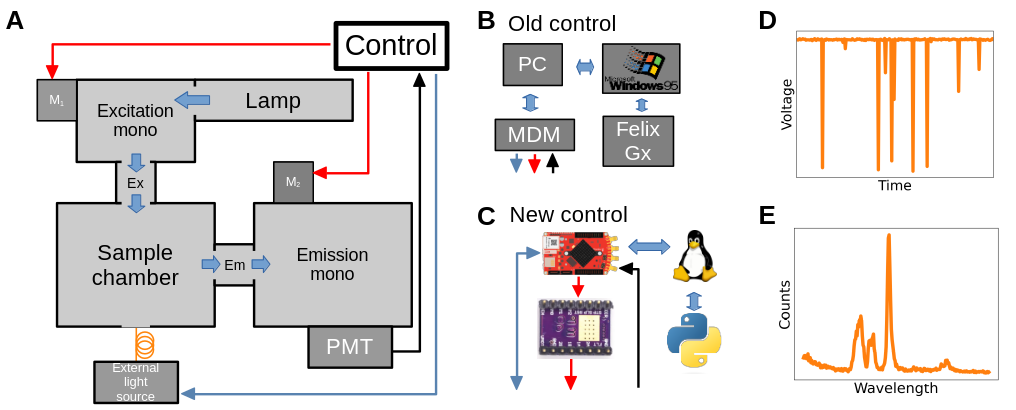
\includegraphics[width=\textwidth]{refurbishment-diagram.png}
     \caption{
    \textbf{Schematic representation of the spectrofluorometer}
    (\textbf{A}) Diagram of the Horiba PTI QuantaMaster hardware. Red arrows represent motors and limit switch connectors, black is BNC, blue is USB and orange represents a fiber optic. The path that light takes inside the spectrometer is represented in thick blue arrows. 
    (\textbf{B}) and (\textbf{C}) Representation of the old and new instrumental control module respectively.
    (\textbf{D}) Representation of the raw signal measured from the PMT detector.
    (\textbf{E}) Spectrum of the sample constructed from the raw signals measured at each wavelength.
    }
     \label{fig:ref-diagram}
\end{figure}

\begin{figure}[h]
     \centering
     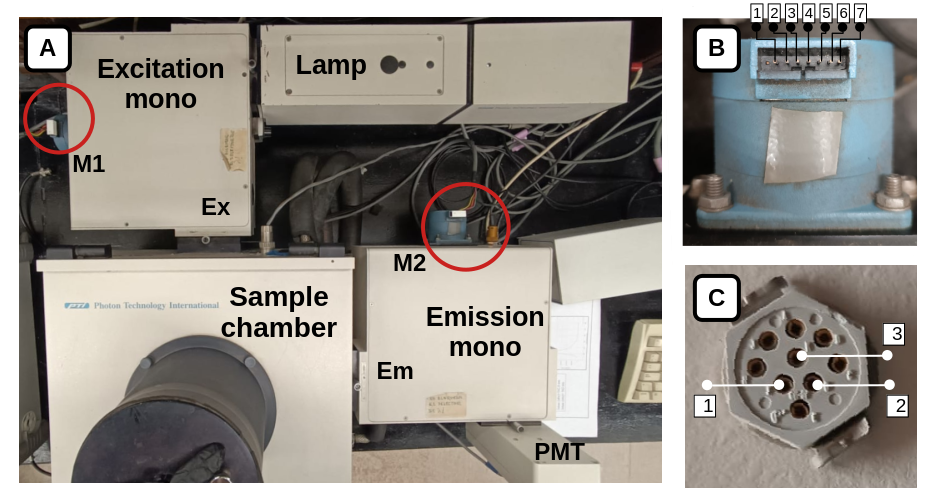
\includegraphics[width=0.9\textwidth]{hardware.png}
     \caption{\textbf{Horiba PTI QuantaMaster 400 picture}. \todo{maybe pasar a apéndice} (\textbf{A}) Picture of the whole spectrometer. Circled in red the monochromators' motors and limit switches. (\textbf{B}) Stepper motors pin diagram. The only used pins for the refurbished version are 1 and 7, and 3 and 5, which correspond to each motor winding respectively. (\textbf{C}) Limit switches pin diagram.}
     \label{fig:hardware}
\end{figure}


\section{Renovación de HoribaPTI QuantaMaster 400}
\subsection{Hardware \todo{quizás es al pedo diferenciar entre hw y sw}}


Qué reemplazamos y con qué nos quedasmos, especificaciones finales

\begin{figure}[h]
     \centering
     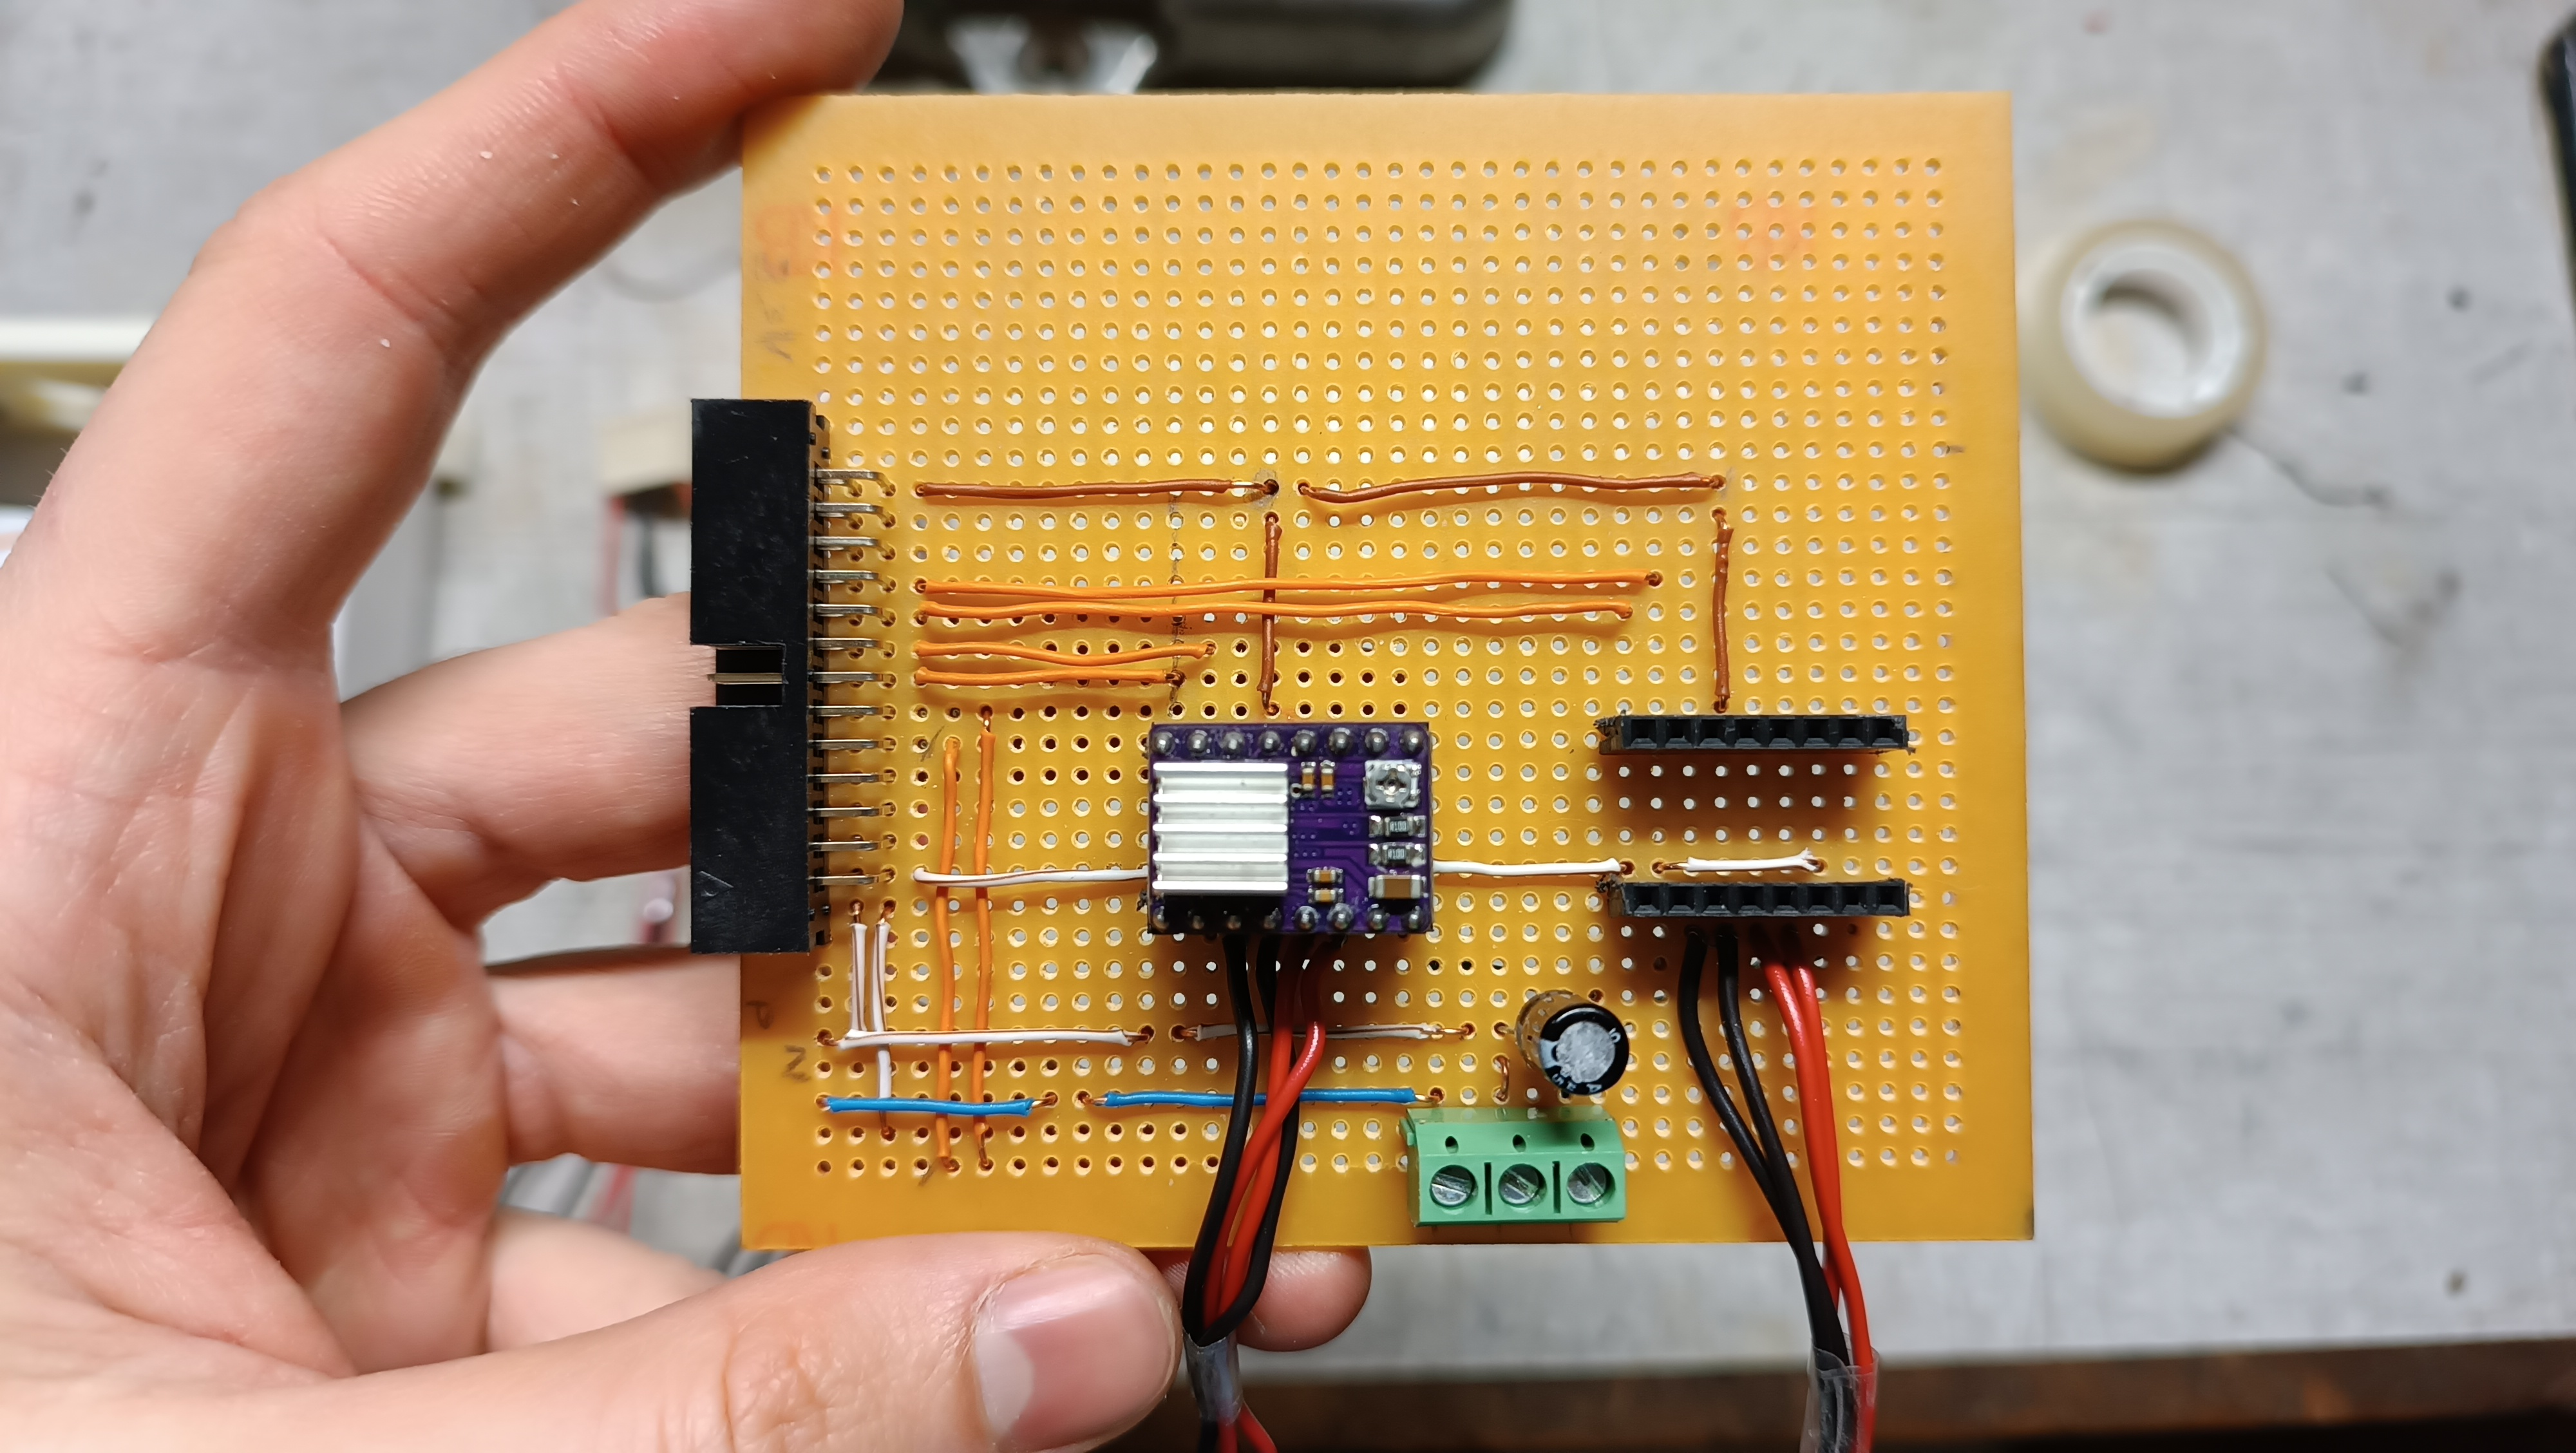
\includegraphics[width=0.9\textwidth]{placa.jpg}
     \caption{\textbf{Horiba PTI QuantaMaster 400 picture}. \todo{maybe pasar a apéndice} (\textbf{A}) Picture of the whole spectrometer. Circled in red the monochromators' motors and limit switches. (\textbf{B}) Stepper motors pin diagram. The only used pins for the refurbished version are 1 and 7, and 3 and 5, which correspond to each motor winding respectively. (\textbf{C}) Limit switches pin diagram.}
     \label{fig:placa}
\end{figure}

\begin{figure}[h]
     \centering
     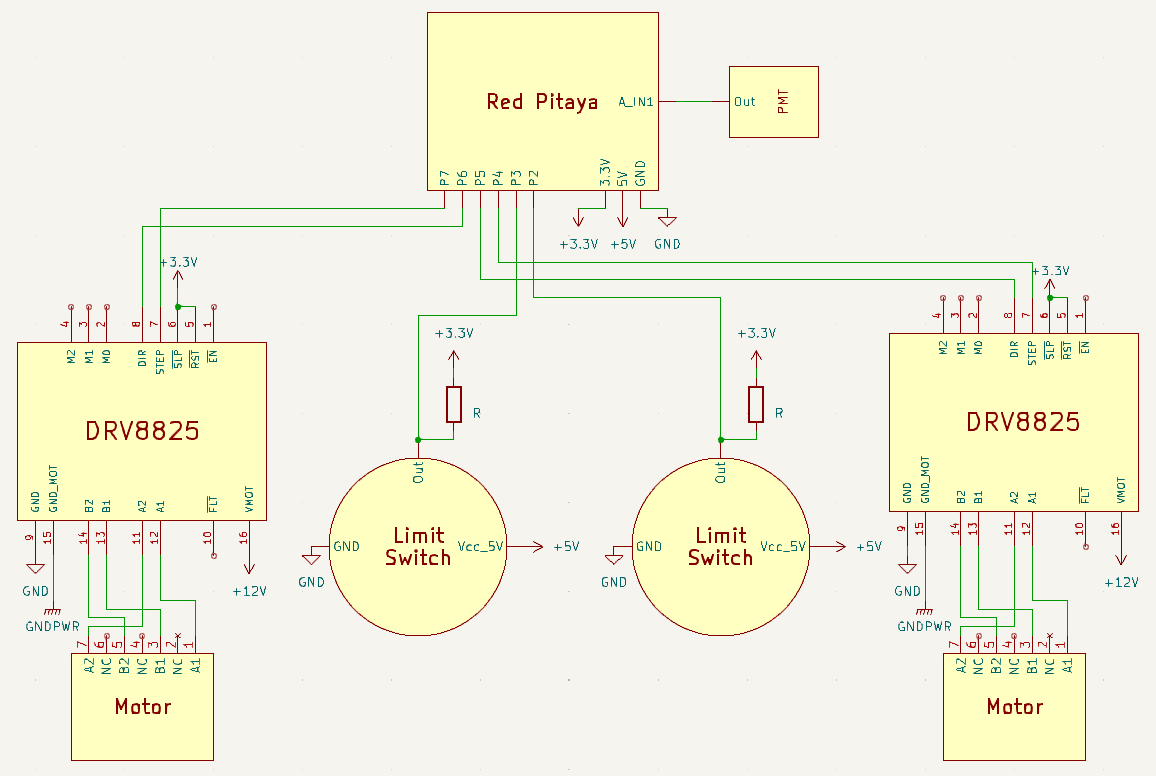
\includegraphics[width=.65\textwidth]{schematic.png}
     \caption{\textbf{Connection diagram}.
     }
     \label{fig:schematic}
\end{figure}

\subsection{Software}



\begin{enumerate}
    \item principios de diseño para desacoplar
    \item API en python
    \item gui
\end{enumerate}

\begin{figure}[h]
     \centering
     \caption{\textbf{Structure of the software}. Each element of the software is ordered from high level (\textbf{top}) to low level (\textbf{bottom}). Inside the dashed line black box In yellow, the two ways the end user can interact with the software. In orange, the refurbished instrument API classes. In red, the RP's hardware API.}
     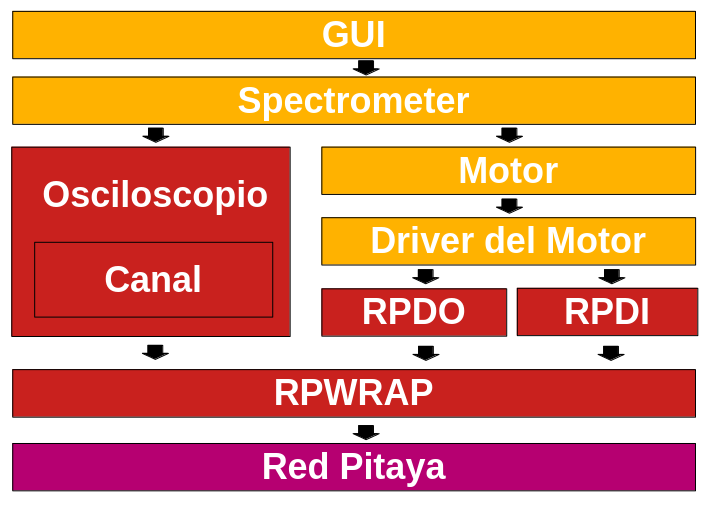
\includegraphics[scale=0.3]{software-diagram.png}
     \label{fig:code}
\end{figure}


\section{Expansión de Horiba PTI QuantaMaster 400 - Medición de tiempos de vida}
\subsection{Hardware}

\begin{enumerate}
    \item Laser de excitación
    \item trigger RP
\end{enumerate}

\subsection{Software}
